\chapter{Computational Study}

This chapter presents our computational study and is structured as follows: Section 5.1 describes the data our experiments are conducted on.  
\section{Data exploration}

The available data set is provided by \cite{Hildebrandt2020_EAT} who created a high-dimensional data model with the RMDP instances originally used in \cite{UlmerRMDP}. It comprises 850.469 samples, 23.341 unique customer locations, a delivery fleet of 15 vehicles and 15 unique restaurant locations. The temporal and spatial distribution of the orders is depicted in figure \ref{fig:dists}. 
\begin{figure}[h]
	\centering
	\subfigure[Request arrival time distribution]{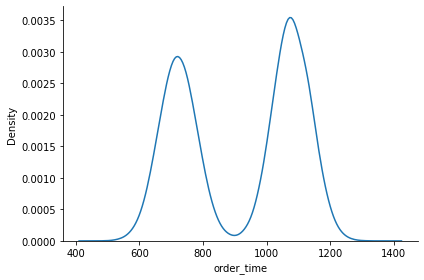
\includegraphics[width=0.49\linewidth]{../Implementation/Plots/order_time_dist.png}}
	\subfigure[Spatial distributions]{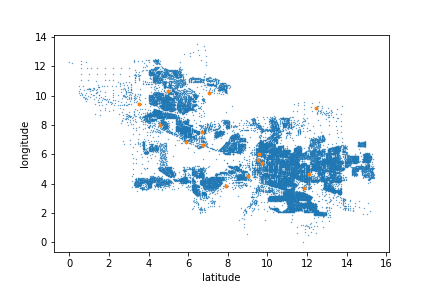
\includegraphics[width=0.49\linewidth]{../Implementation/Plots/spatial_dist.png}}
	\caption{Spatial and temporal distributions}
	\label{fig:dists}
\end{figure}

Panel (a) of figure \ref{fig:dists} shows the order behaviour of customers. The x-axis denotes the day time in minutes, the y-axis denotes the relative frequency of incoming customer orders for a given day time on the y-axis. We can observe that the order time behaviour across all customers follows a bimodal gaussian distribution. The order frequency peaks at around 12:00 a.m (roughly 700 minutes of day time) and again around 6.00 p.m (roughly 1100 minutes of day time). This indicates that the probability of an order taking place during lunch or dinner time is relatively high.  
Panel (b) of figure \ref{fig:dists} shows the spatial distribution of customer and restaurant locations. The x-axis depicts the 

\begin{figure}[h]
	\centering
	\subfigure[]{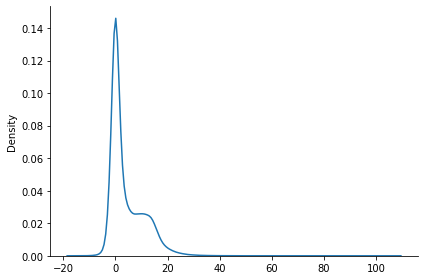
\includegraphics[width=0.49\linewidth]{../Implementation/Plots/delivery_delay.png}}
	\subfigure[Temporal distributions]{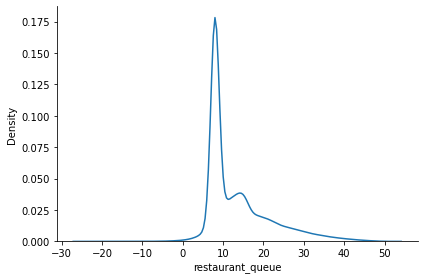
\includegraphics[width=0.49\linewidth]{../Implementation/Plots/prep_time.png}}
	\caption{Spatial and temporal distributions}
	\label{fig:prepdelay}
\end{figure}

Panel (a) of figure \ref{fig:predelay} shows the distribution of delivery delay times in minutes for all requests in the data. We notice that deliveries happen on time for 


 
\section{Experiment 1: Sample Size tests}


\section{Experiment 2: Hyperparameter Optimization}

This section presents the hyperparameter optimization (HPO) experiments conducted for GBDTs, RFs, and the neural network architecture presented in section \ref{sec:nn}. 
We use \textit{Optuna} to conduct our HPO experiments, a popular HPO framework presented in \cite{akiba2019optuna}. \textit{Optuna} provides a simple implementation design that allows us to analyze evaluated parameters from different points of view. 
The optimizations were conducted on both the crafted data set and the raw data set. Concretely, we will proceed as follows: First, we will present the hyperparameters we decided to include in the HPO to then in turn present the optimal hyperparameter values resulting from the experiment and explore the predictive power of different parametrizations. By that, we hope to get a fine-tuned model that maximizes prediction quality on one hand, and intuition for parametrization on the other. Secondly, we will use the \textit{optuna} implementation of the \textit{fANOVA} evaluation algorithm presented in \cite{fANOVA} to determine hyperparameter importances. Thereby, we can assess which parameters impact the model significantly and which parameters are less significant, and especially how the importances differ for the two data sets. Lastly, we will examine interdependencies between the evaluated hyperparameters. 
 
\subsection{Tree-based Ensembles}

In this section, we will conduct HPO experiments for the tree-based ensembles. We are going to start with the optimization and analysis for GBDT.
For GBDT, we decided to optimize following parameters and set the search spaces for each them as follows:
\begin{description}[font=$\bullet$\scshape\bfseries]
	\item $ \text{learning\_rate} \in [0.01, 0.05] $  in steps of 0.001.
	\item $ \text{max\_depth} \in [5, 100] $ in steps of 0.001.
	\item $ \text{feature\_fraction} \in [0.1, 1.0] $ in steps of 0.01.
	\item $ \text{feature\_fraction\_bynode} \in [0.3, 1.0] $ in steps of 0.01
	\item $ \text{num\_leaves} \in [20, 300] $ in steps of 1
	\item $ \text{min\_child\_samples} \in [10, 400] $ in steps of 1.
	\item $ \text{subsample\_freq} \in [1, 10] $ in steps of 1.
	\item $ \text{subsample} \in [0.3, 1.0] $ in steps of 0.01.
\end{description}
The selection of parameter search spaces is the result of trial-and-error since the determination of parameter values respectively parameter search spaces has to be determined at least partly in a manual, heuristic fashion. Detailed explanations of the considered parameters for GBDT can be found under \url{https://lightgbm.readthedocs.io/en/latest/Parameters.html}. 

%\begin{figure}[h]
%	\centering
%	\includegraphics[width=\linewidth]{figures/HPO/GBDT_HPO_Raw.png}
%	\caption{Hyperparameter Importances for GBDT on raw data}
%	\label{fig:GBDT_HPO_Raw}
%\end{figure}
%\begin{figure}[h]
%	\centering
%	\includegraphics[width=\linewidth]{figures/HPO/GBDT_HPO_Crafted.png}
%	\caption{Hyperparameter Importances for GBDT on crafted data model}
%	\label{fig:GBDT_HPO_Crafted}
%\end{figure}
\begin{figure}[h]
	\centering
	\subfigure{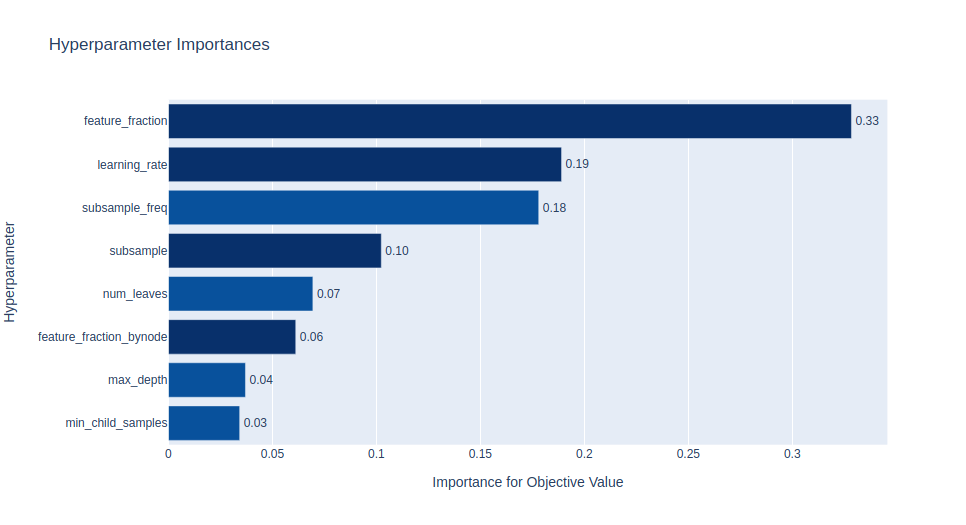
\includegraphics[width=0.49\linewidth]{figures/HPO/GBDT_HPO_Crafted_Importances.png}}
	\subfigure{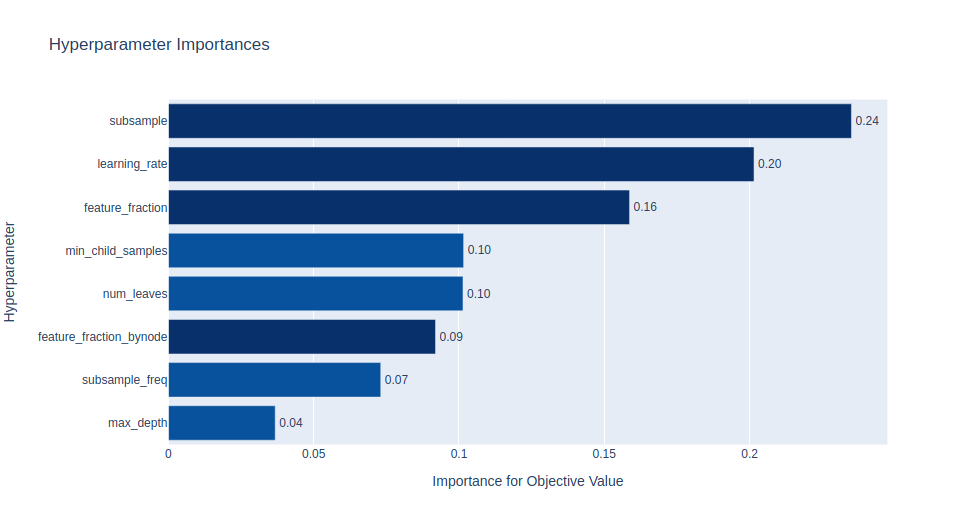
\includegraphics[width=0.49\linewidth]{figures/HPO/GBDT_HPO_Raw_Importances.png}}
	\caption{Hyperparameter Importances for GBDT on each dataset}
	\label{fig:GBDT_HPO_Crafted}
\end{figure}
\begin{figure}[h]
	\centering
	\subfigure{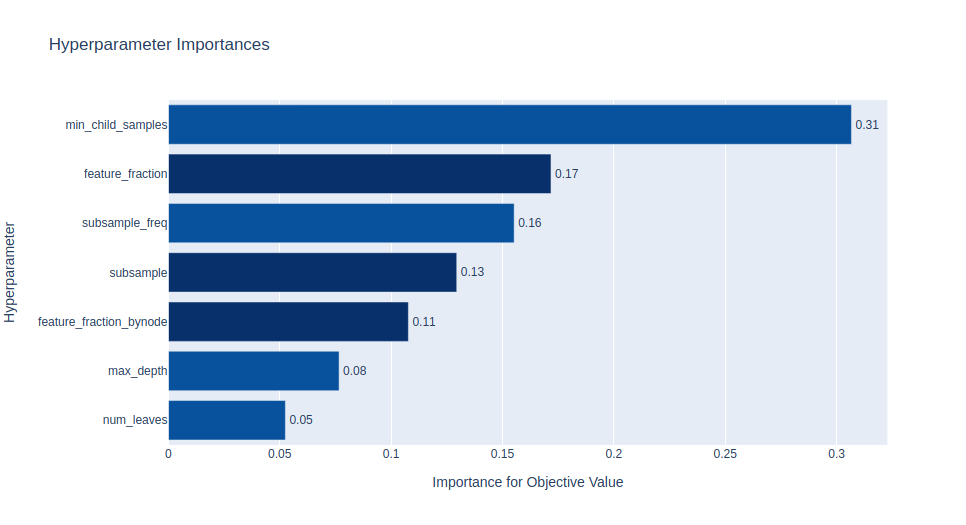
\includegraphics[width=0.49\linewidth]{figures/HPO/RF_HPO_Crafted_Importances.png}}
	\subfigure{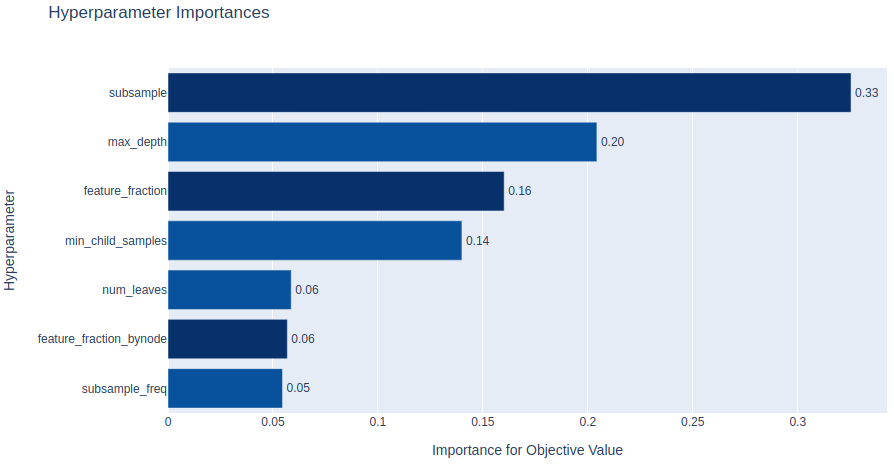
\includegraphics[width=0.49\linewidth]{figures/HPO/RF_HPO_Raw_Importances.png}}
	\caption{Hyperparameter Importances for RF on each dataset}
	\label{fig:GBDT_HPO_Crafted}
\end{figure}

\section{Experiment 3: Introducing noise}







